% SI - Figure 1 Example route with data
\begin{figure}[htb]
\centering
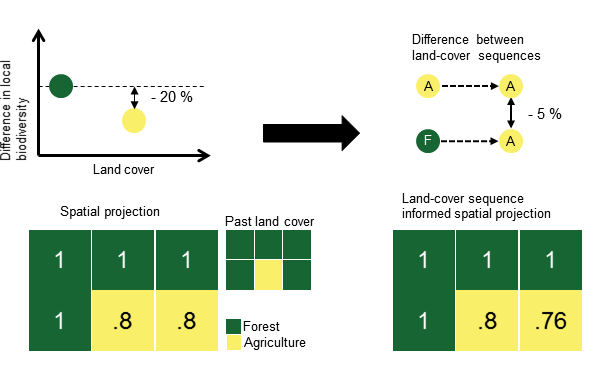
\includegraphics[width=1\textwidth]{chapter5/SI01}
\caption{Annual Landsat composite for a single year (2018) and route (RTENO: \texttt{89020}, Routename: \textit{Wapato} in the State of Washington) showing the month with the greenest EVI value in the period $20^th$ March to $20^th$ June. }
\label{SI05_01}
\end{figure}

% SI - Figure 2 Missing data
\begin{figure}[htb]
\centering
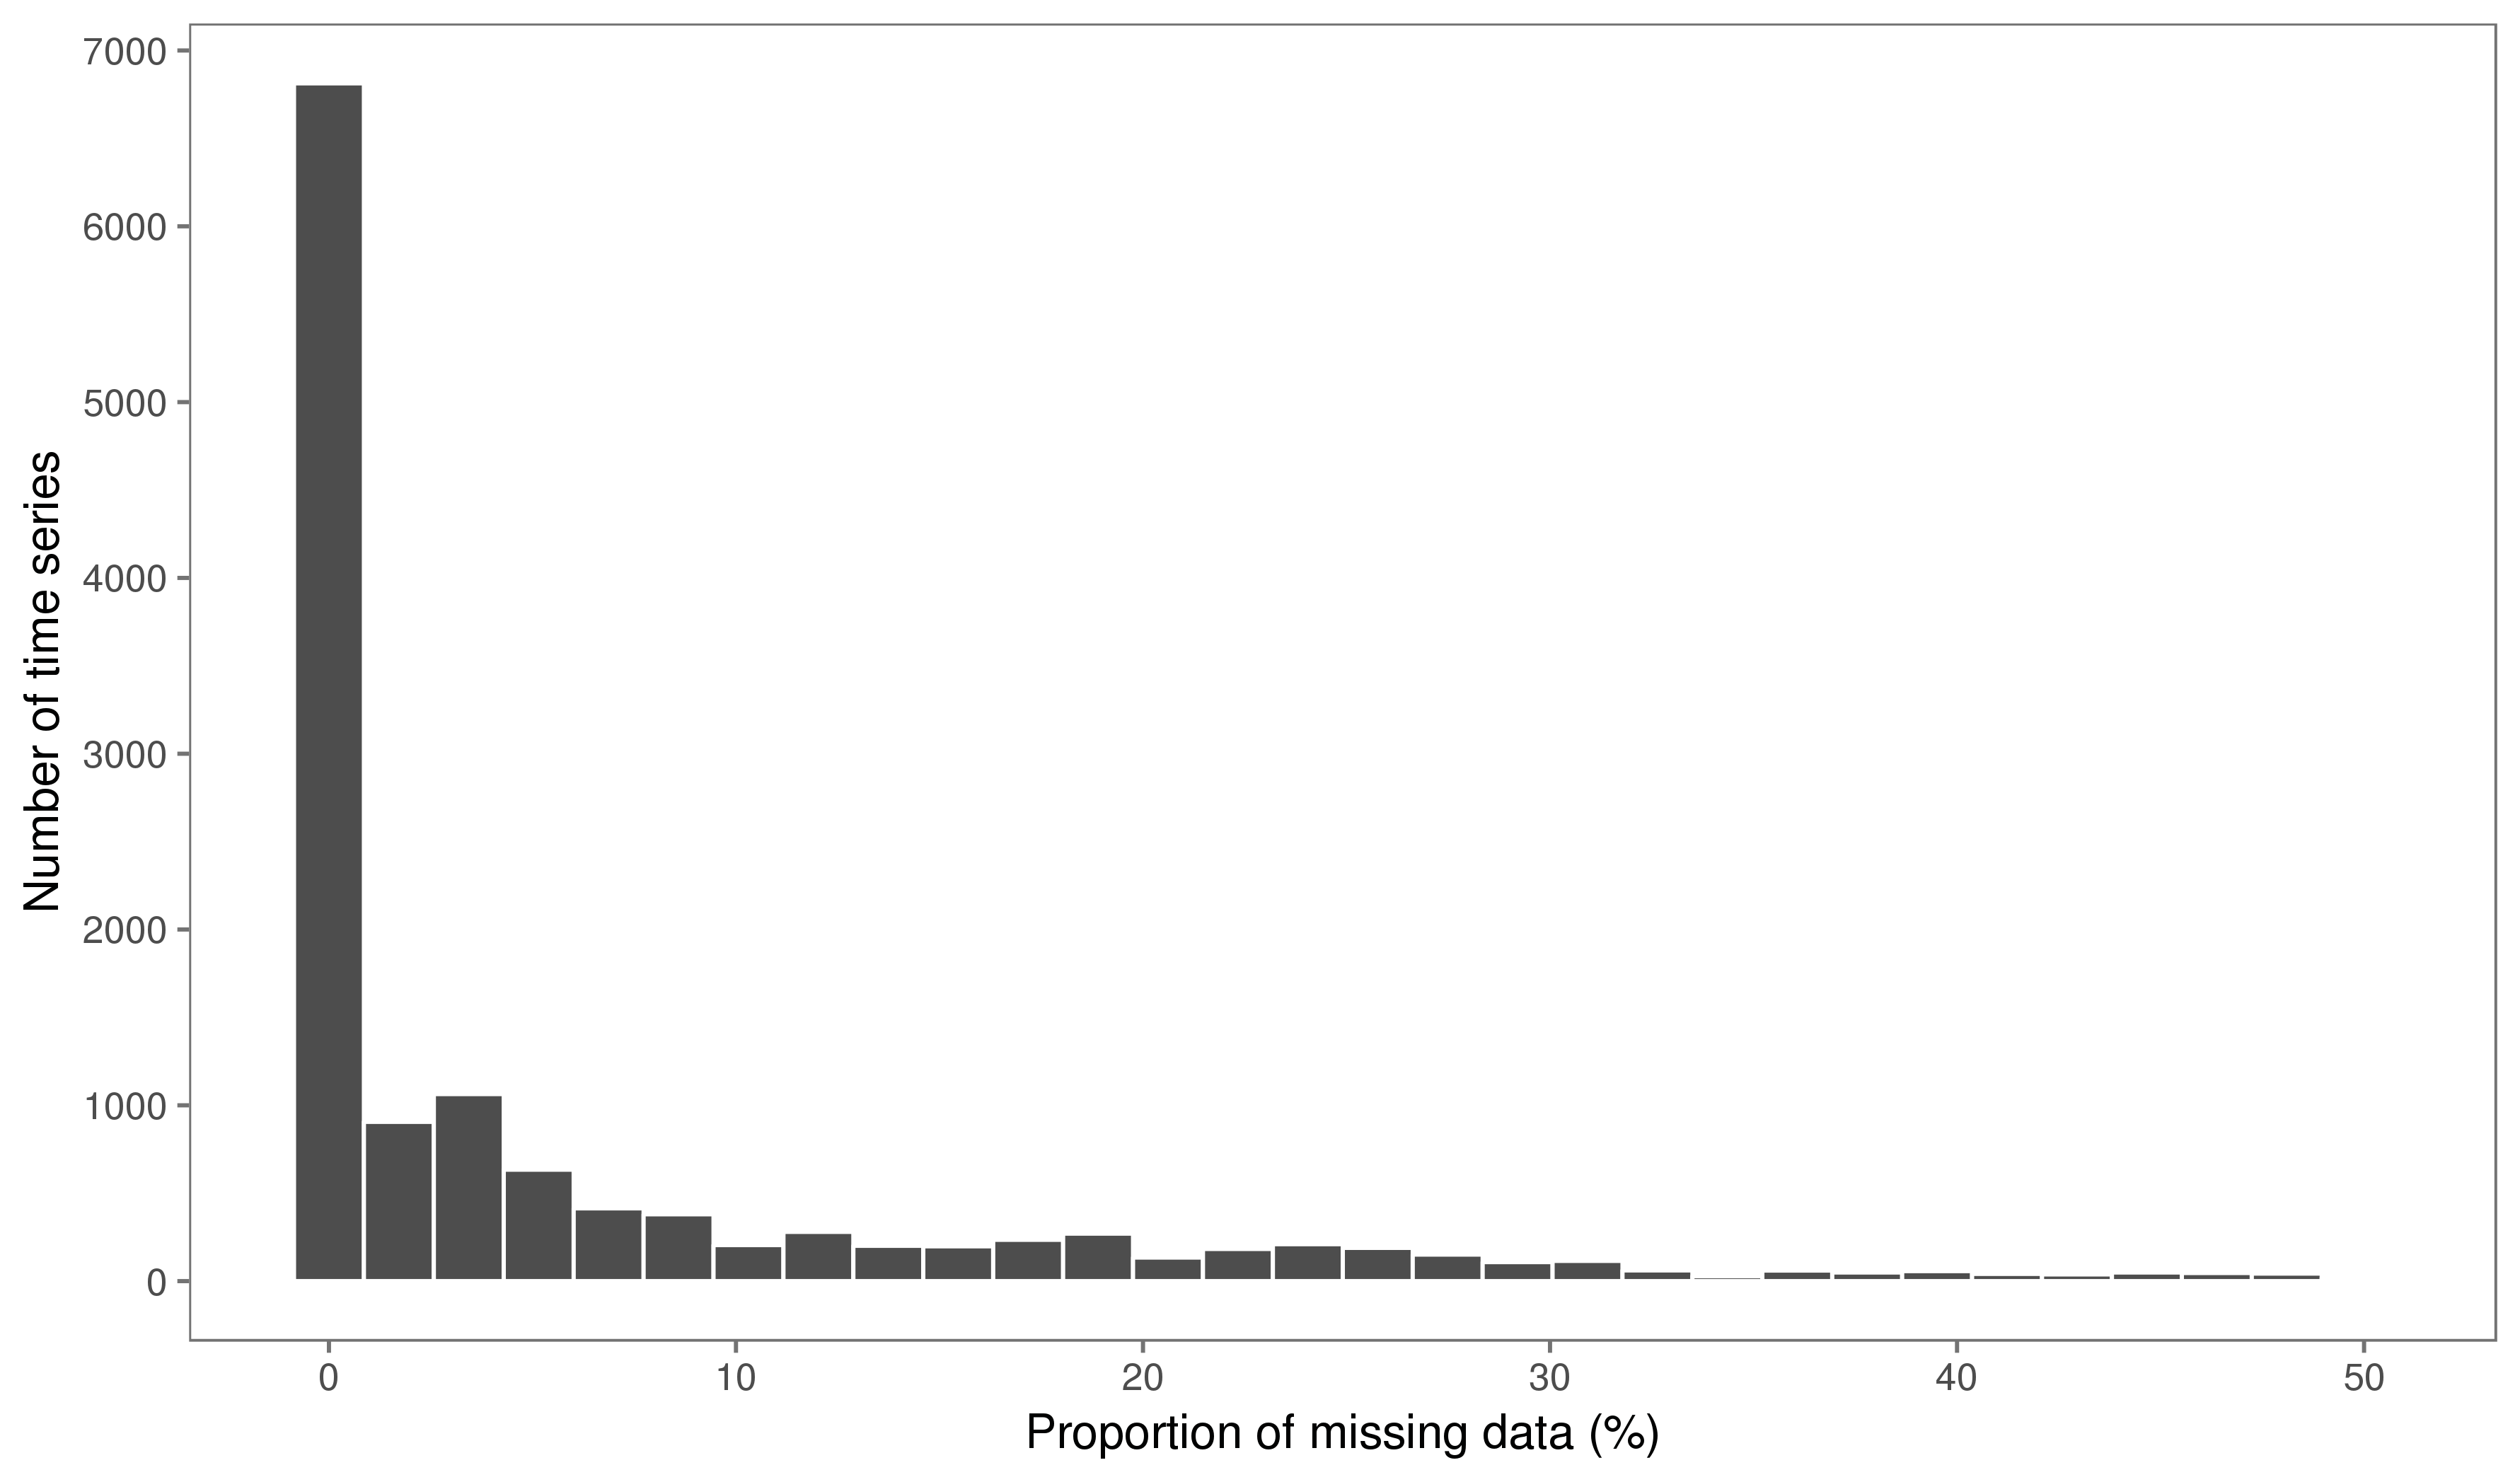
\includegraphics[width=1\textwidth]{chapter5/SI02}
\caption{(\textbf{a}) Average proportion of missing Landsat data across years for all routes with the median (1.06\%) indicated (dotted line). (\textbf{b}) Map showing each BBS Route coloured by the average proportion (\%) of missing data across years.}
\label{SI05_02}
\end{figure}

% SI - Figure 3-4 Model checks
\begin{figure}[htb]
\centering
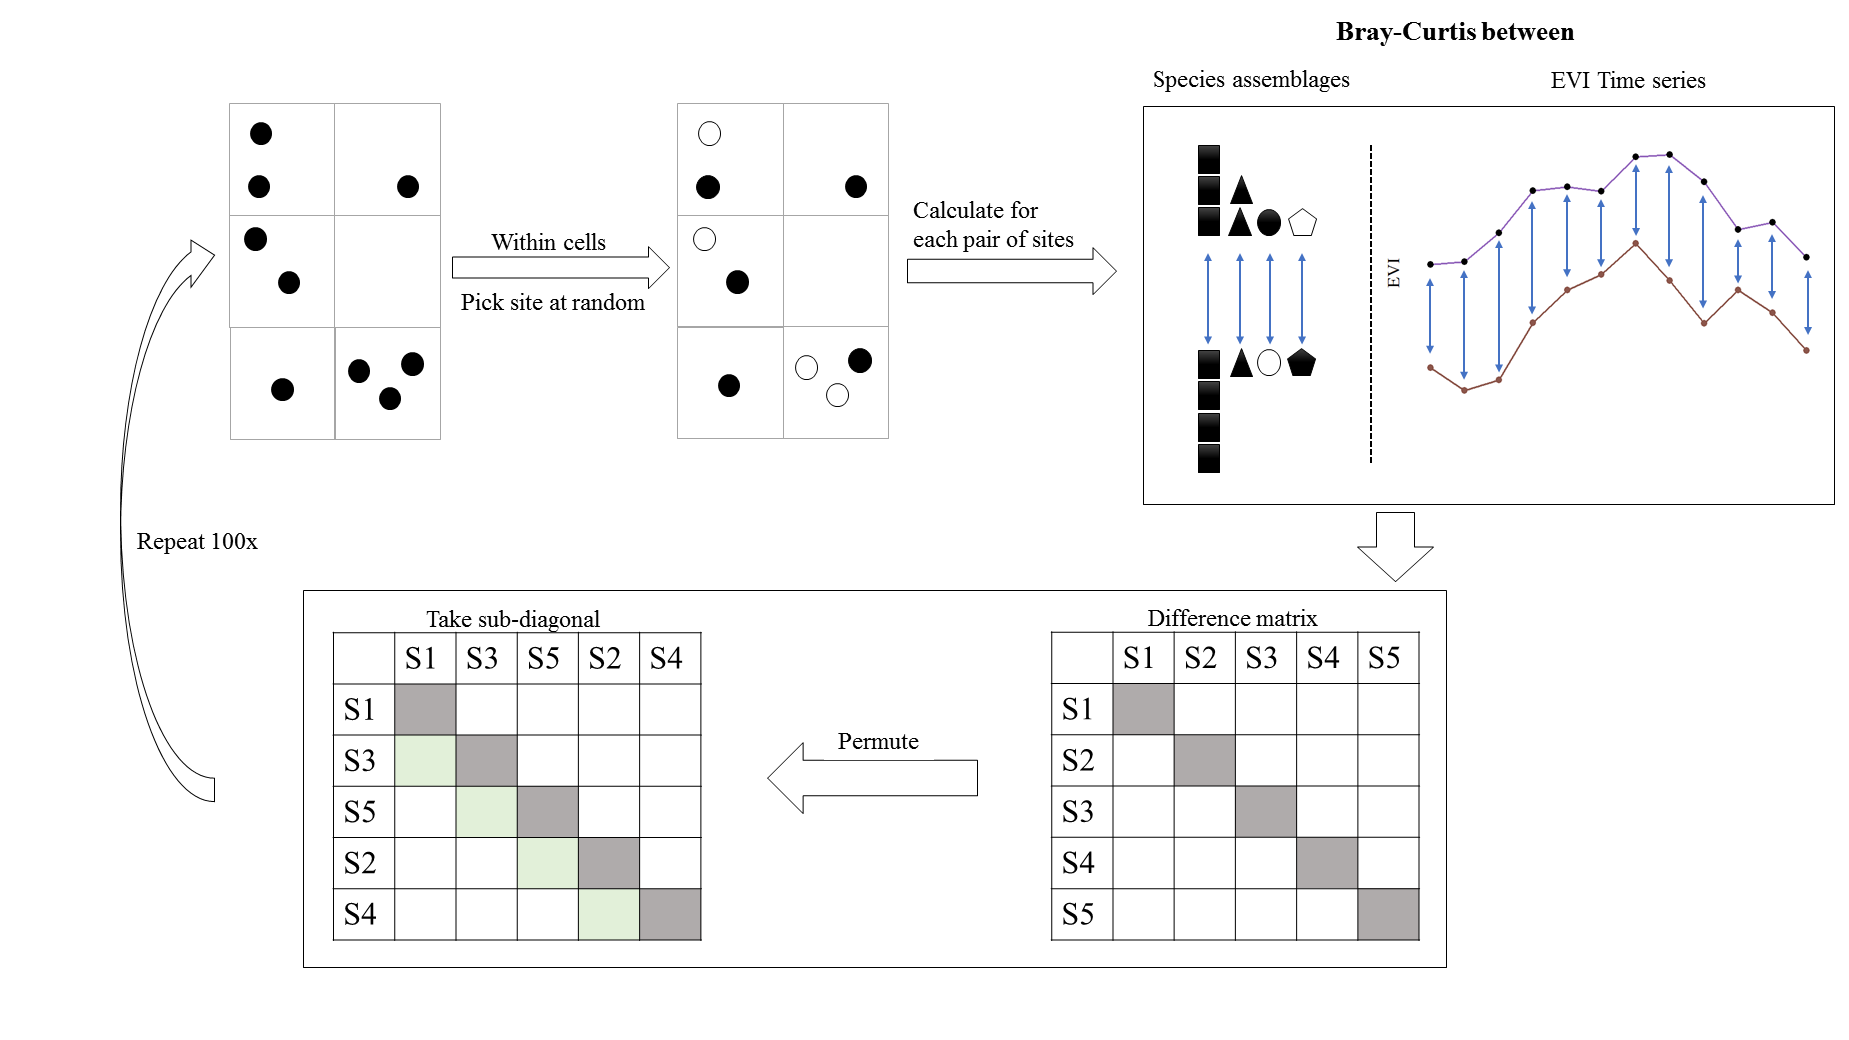
\includegraphics[width=1\textwidth]{chapter5/SI03}
\caption{Model diagnostics of the full model (see \ref{C05_0205}) for the geometric mean of relative abundances (GM).}
\label{SI05_03}
\end{figure}

\begin{figure}[htb]
\centering
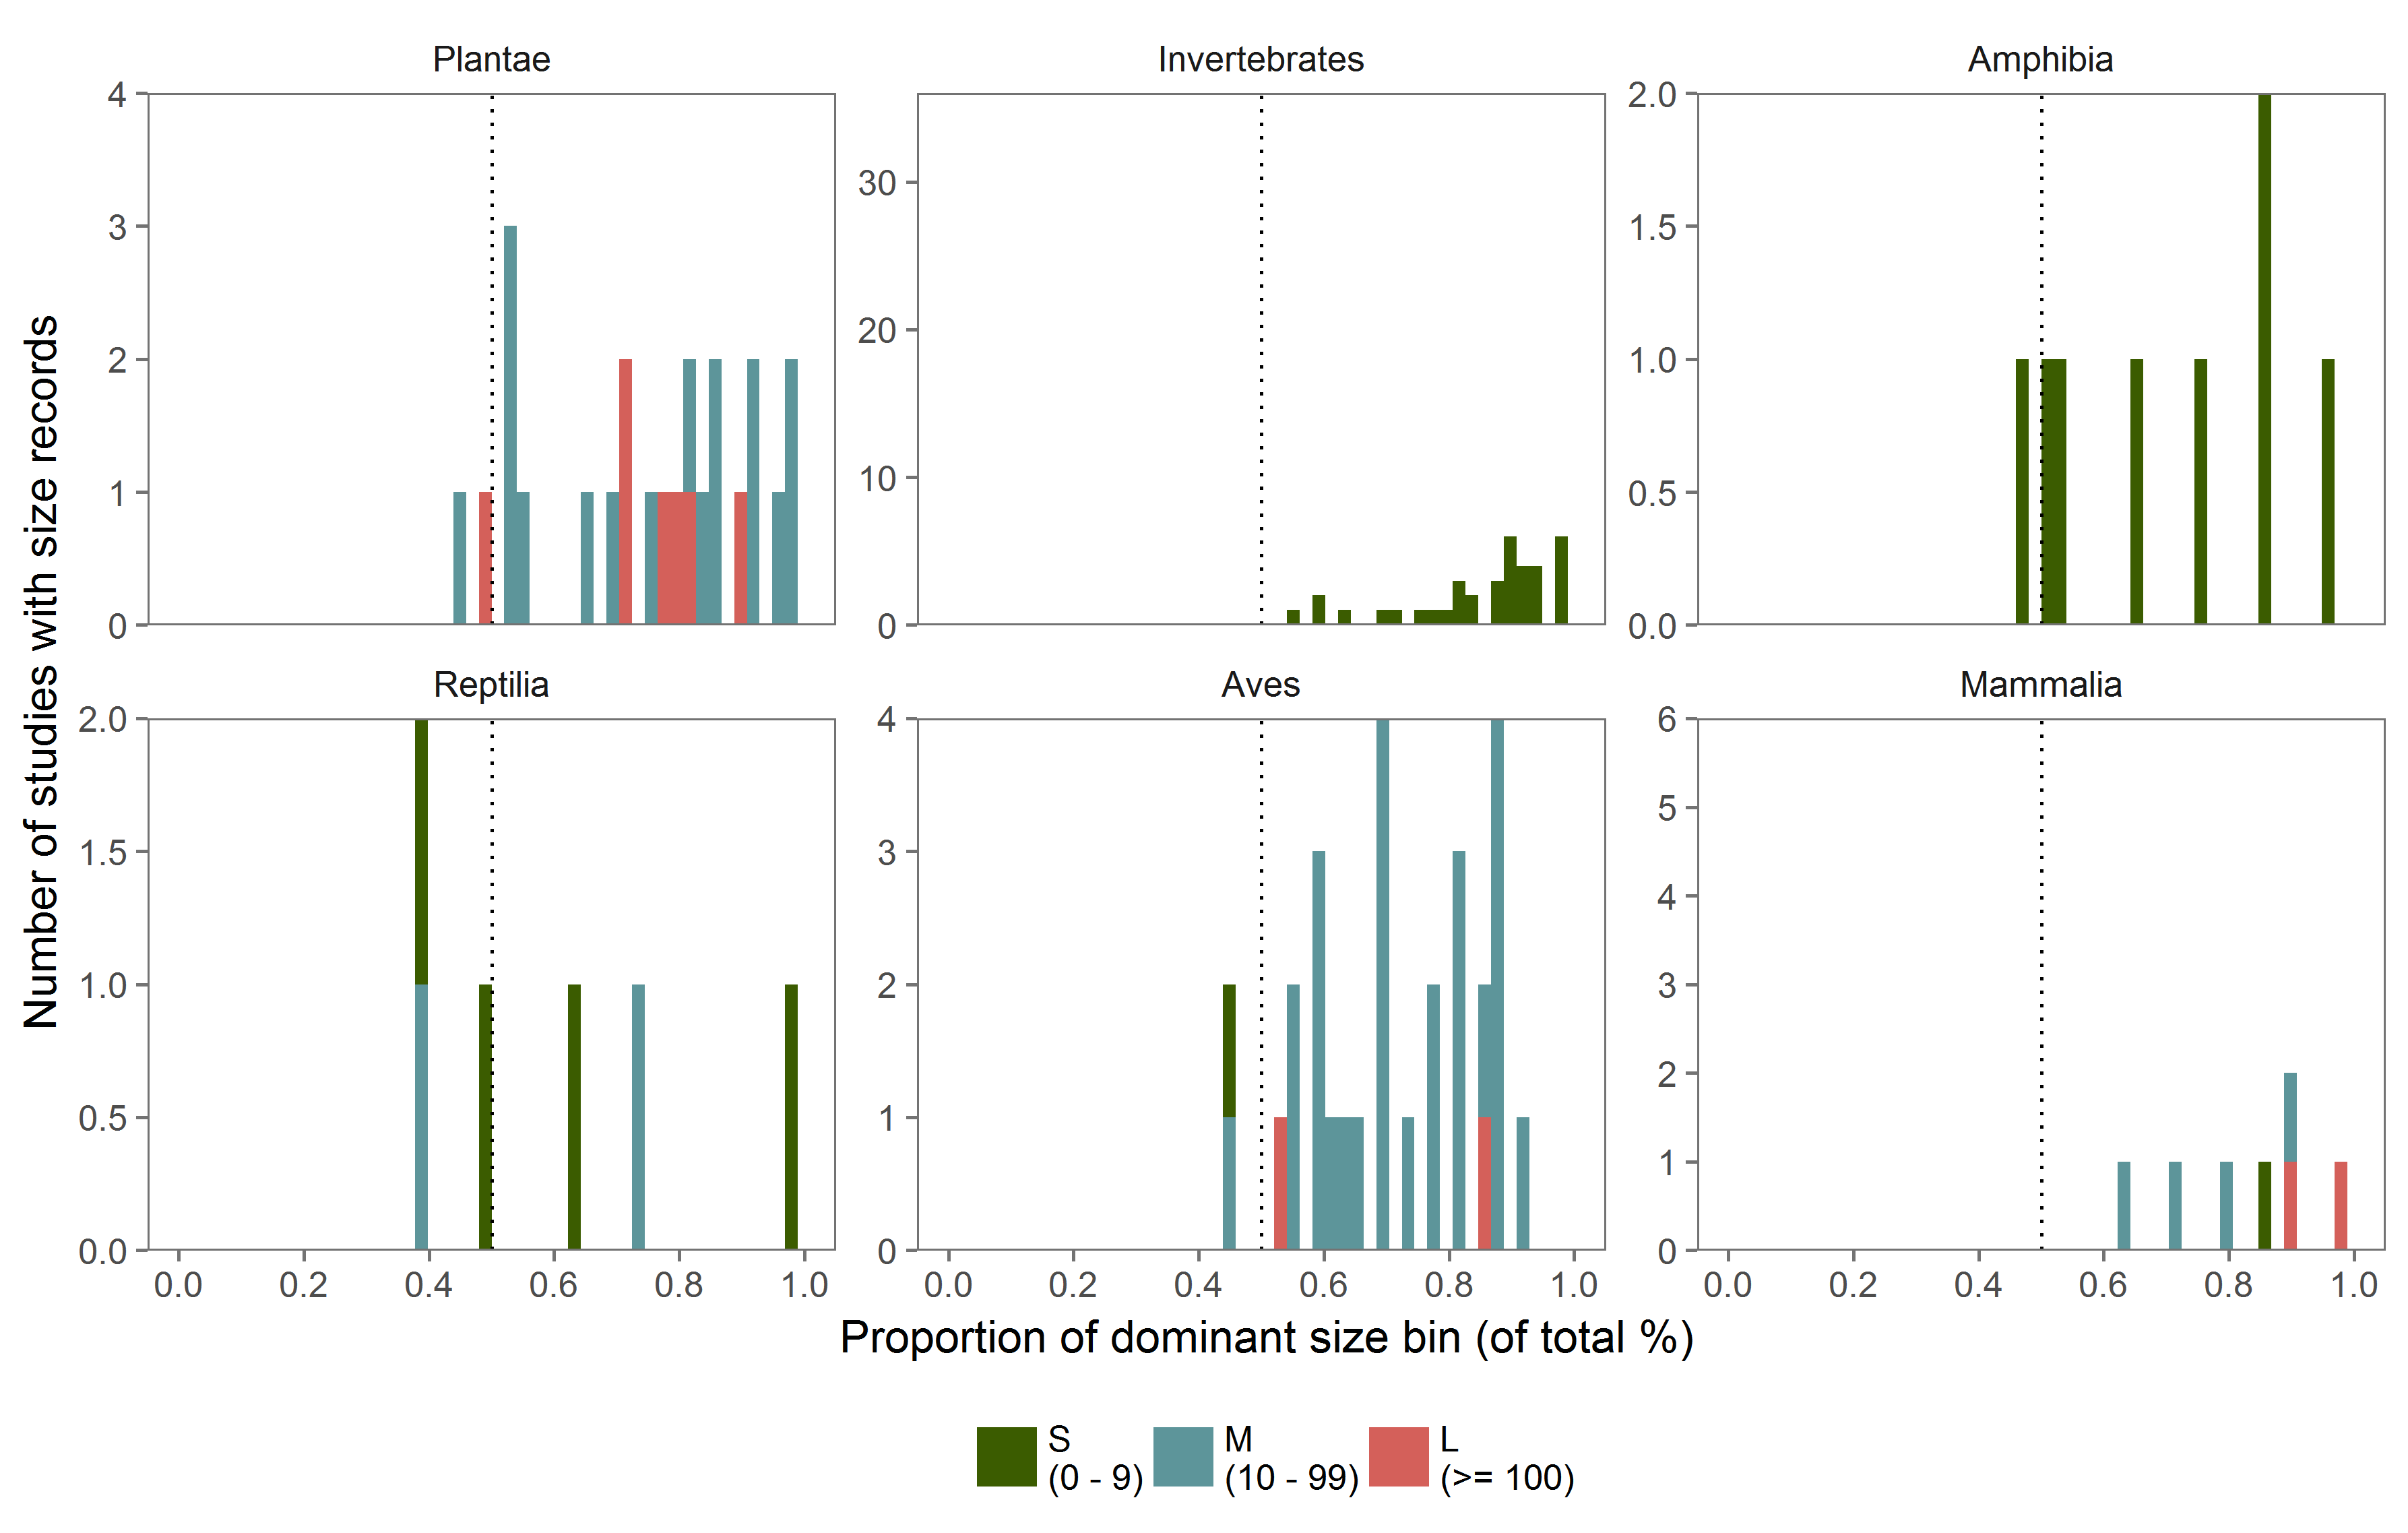
\includegraphics[width=1\textwidth]{chapter5/SI04}
\caption{Model diagnostics of the full model (see \ref{C05_0205}) for the progressive Bray-Curtis index (pBC).}
\label{SI05_04}
\end{figure}